% Options for packages loaded elsewhere
\PassOptionsToPackage{unicode}{hyperref}
\PassOptionsToPackage{hyphens}{url}
%
\documentclass[
  12pt,
  a4paper,
  DIV=11,
  numbers=noendperiod]{scrreprt}

\usepackage{amsmath,amssymb}
\usepackage{setspace}
\usepackage{iftex}
\ifPDFTeX
  \usepackage[T1]{fontenc}
  \usepackage[utf8]{inputenc}
  \usepackage{textcomp} % provide euro and other symbols
\else % if luatex or xetex
  \usepackage{unicode-math}
  \defaultfontfeatures{Scale=MatchLowercase}
  \defaultfontfeatures[\rmfamily]{Ligatures=TeX,Scale=1}
\fi
\usepackage{lmodern}
\ifPDFTeX\else  
    % xetex/luatex font selection
\fi
% Use upquote if available, for straight quotes in verbatim environments
\IfFileExists{upquote.sty}{\usepackage{upquote}}{}
\IfFileExists{microtype.sty}{% use microtype if available
  \usepackage[]{microtype}
  \UseMicrotypeSet[protrusion]{basicmath} % disable protrusion for tt fonts
}{}
\usepackage{xcolor}
\setlength{\emergencystretch}{3em} % prevent overfull lines
\setcounter{secnumdepth}{5}
% Make \paragraph and \subparagraph free-standing
\ifx\paragraph\undefined\else
  \let\oldparagraph\paragraph
  \renewcommand{\paragraph}[1]{\oldparagraph{#1}\mbox{}}
\fi
\ifx\subparagraph\undefined\else
  \let\oldsubparagraph\subparagraph
  \renewcommand{\subparagraph}[1]{\oldsubparagraph{#1}\mbox{}}
\fi


\providecommand{\tightlist}{%
  \setlength{\itemsep}{0pt}\setlength{\parskip}{0pt}}\usepackage{longtable,booktabs,array}
\usepackage{calc} % for calculating minipage widths
% Correct order of tables after \paragraph or \subparagraph
\usepackage{etoolbox}
\makeatletter
\patchcmd\longtable{\par}{\if@noskipsec\mbox{}\fi\par}{}{}
\makeatother
% Allow footnotes in longtable head/foot
\IfFileExists{footnotehyper.sty}{\usepackage{footnotehyper}}{\usepackage{footnote}}
\makesavenoteenv{longtable}
\usepackage{graphicx}
\makeatletter
\def\maxwidth{\ifdim\Gin@nat@width>\linewidth\linewidth\else\Gin@nat@width\fi}
\def\maxheight{\ifdim\Gin@nat@height>\textheight\textheight\else\Gin@nat@height\fi}
\makeatother
% Scale images if necessary, so that they will not overflow the page
% margins by default, and it is still possible to overwrite the defaults
% using explicit options in \includegraphics[width, height, ...]{}
\setkeys{Gin}{width=\maxwidth,height=\maxheight,keepaspectratio}
% Set default figure placement to htbp
\makeatletter
\def\fps@figure{htbp}
\makeatother

\usepackage{indentfirst}
\usepackage{float}
\floatplacement{figure}{H}
\IfFileExists{plex-otf.sty}{
  %% Full TeXlive
  \usepackage[
    % math,
    RM={Scale=0.94},SS={Scale=0.94},SScon={Scale=0.94},TT={Scale=MatchLowercase,FakeStretch=0.9},
    DefaultFeatures={Ligatures=Common}
  ]{plex-otf}
  % \usepackage[Scale=MatchUppercase]{juliamono}
}{
  %% TinyTeX
  \usepackage{libertine}
}
\KOMAoption{captions}{tableheading}
\makeatletter
\@ifpackageloaded{caption}{}{\usepackage{caption}}
\AtBeginDocument{%
\ifdefined\contentsname
  \renewcommand*\contentsname{Содержание}
\else
  \newcommand\contentsname{Содержание}
\fi
\ifdefined\listfigurename
  \renewcommand*\listfigurename{Список иллюстраций}
\else
  \newcommand\listfigurename{Список иллюстраций}
\fi
\ifdefined\listtablename
  \renewcommand*\listtablename{Список таблиц}
\else
  \newcommand\listtablename{Список таблиц}
\fi
\ifdefined\figurename
  \renewcommand*\figurename{Рисунок}
\else
  \newcommand\figurename{Рисунок}
\fi
\ifdefined\tablename
  \renewcommand*\tablename{Таблица}
\else
  \newcommand\tablename{Таблица}
\fi
}
\@ifpackageloaded{float}{}{\usepackage{float}}
\floatstyle{ruled}
\@ifundefined{c@chapter}{\newfloat{codelisting}{h}{lop}}{\newfloat{codelisting}{h}{lop}[chapter]}
\floatname{codelisting}{Список}
\newcommand*\listoflistings{\listof{codelisting}{Листинги}}
\makeatother
\makeatletter
\makeatother
\makeatletter
\@ifpackageloaded{caption}{}{\usepackage{caption}}
\@ifpackageloaded{subcaption}{}{\usepackage{subcaption}}
\makeatother
\ifLuaTeX
\usepackage[bidi=basic]{babel}
\else
\usepackage[bidi=default]{babel}
\fi
\babelprovide[main,import]{russian}
\babelprovide[import]{english}
% get rid of language-specific shorthands (see #6817):
\let\LanguageShortHands\languageshorthands
\def\languageshorthands#1{}
\ifLuaTeX
  \usepackage{selnolig}  % disable illegal ligatures
\fi
\usepackage[style=gost-numeric,backend=biber,langhook=extras,autolang=other*]{biblatex}
\addbibresource{bib/cite.bib}
\usepackage{csquotes}
\usepackage{bookmark}

\IfFileExists{xurl.sty}{\usepackage{xurl}}{} % add URL line breaks if available
\urlstyle{same} % disable monospaced font for URLs
\hypersetup{
  pdftitle={Отчёта по лабораторной работе 7},
  pdfauthor={Нджову Нелиа},
  pdflang={ru-RU},
  hidelinks,
  pdfcreator={LaTeX via pandoc}}

\title{Отчёта по лабораторной работе 7}
\usepackage{etoolbox}
\makeatletter
\providecommand{\subtitle}[1]{% add subtitle to \maketitle
  \apptocmd{\@title}{\par {\large #1 \par}}{}{}
}
\makeatother
\subtitle{Математическое моделирование}
\author{Нджову Нелиа}
\date{}

\begin{document}
\maketitle

\renewcommand*\contentsname{Содержание}
{
\setcounter{tocdepth}{1}
\tableofcontents
}
\listoffigures
\listoftables
\setstretch{1.5}
\chapter{Цель
работы}\label{ux446ux435ux43bux44c-ux440ux430ux431ux43eux442ux44b}

Целью данной лабораторной работы является построение математической
модели Эффективность рекламы.

\chapter{Задание}\label{ux437ux430ux434ux430ux43dux438ux435}

\textbf{Вариант 64}

Постройте график распространения рекламы, математическая модель которой
описывается следующим уравнением:

\begin{enumerate}
\def\labelenumi{\arabic{enumi}.}
\item
  \(\frac{dn}{dt} = (0.605 + 0.000015n(t))(N - n(t))\)
\item
  \(\frac{dn}{dt} = (0.000025 + 0.205n(t))(N - n(t))\)
\item
  \(\frac{dn}{dt} = (0.05sin(t) + 0.31cos(t)n(t))(N - n(t))\)
\end{enumerate}

При этом объем аудитории N = 1515, в начальный момент о товаре знает 12
человек. Для случая 2 определите в какой момент времени скорость
распространения рекламы будет иметь максимальное значение.

\chapter{Теоретическое
введение}\label{ux442ux435ux43eux440ux435ux442ux438ux447ux435ux441ux43aux43eux435-ux432ux432ux435ux434ux435ux43dux438ux435}

\textbf{Эффективность рекламы}

Организуется рекламная кампания нового товара или услуги. Необходимо,
чтобы прибыль будущих продаж с избытком покрывала издержки на рекламу.
Вначале расходы могут превышать прибыль, поскольку лишь малая часть
потенциальных покупателей будет информирована о новинке. Затем, при
увеличении числа продаж, возрастает и прибыль, и, наконец, наступит
момент, когда рынок насытиться, и рекламировать товар станет
бесполезным.

Предположим, что торговыми учреждениями реализуется некоторая продукция,
о которой в момент времениt из числа потенциальных покупателей N знает
лишьn покупателей. Для ускорения сбыта продукции запускается реклама по
радио, телевидению и других средств массовой информации. После запуска
рекламной кампании информация о продукции начнет распространяться среди
потенциальных покупателей путем общения друг с другом. Таким образом,
после запуска рекламных объявлений скорость изменения числа знающих о
продукции людей пропорциональна как числу знающих о товаре покупателей,
так и числу покупателей о нем не знающих

Модель рекламной кампании описывается следующими величинами. Считаем,
что dn/dt - скорость изменения со временем числа потребителей, узнавших
о товаре и готовых его купить,t - время, прошедшее с начала рекламной
кампании,n(t) - число уже информированных клиентов. Эта величина
пропорциональна числу покупателей, еще не знающих о нем, это описывается
следующим образом: \(a_1(t)(N - n(t))\), где N - общее число
потенциальных платежеспособных покупателей, \(a_1(t) > 0\) -
характеризует интенсивность рекламной кампании (зависит от затрат на
рекламу в данный момент времени). Помимо этого, узнавшие о товаре
потребители также распространяют полученную информацию среди
потенциальных покупателей, не знающих о нем (в этом случае работает т.н.
сарафанное радио). Этот вклад в рекламу описывается величиной
\(a_2(t)n(t)(N - n(t))\), эта величина увеличивается с увеличением
потребителей узнавших о товаре. Математическая модель распространения
рекламы описывается уравнением:

\[
\frac{dn}{dt} = (a_1(t) + a_2(t)n(t))(N - n(t))
\]

\chapter{Выполнение лабораторной
работы}\label{ux432ux44bux43fux43eux43bux43dux435ux43dux438ux435-ux43bux430ux431ux43eux440ux430ux442ux43eux440ux43dux43eux439-ux440ux430ux431ux43eux442ux44b}

\section{Реализация в
Julia}\label{ux440ux435ux430ux43bux438ux437ux430ux446ux438ux44f-ux432-julia}

Давайте определим функцию для решения модели эффективности рекламы. Для
каждого случая мы используем разные интервалы интеграции, а также задаем
начальное значение интеграции и параметры модели. Мы зададим начальные
условия и функции для трех случаев(рис.1)

\begin{figure}

\centering{


\includegraphics[width=0.7\textwidth,height=\textheight]{image/pic7.png}

}

\caption{\label{fig-001}Реализация в Julia}

\end{figure}%

Найдем решение для первого случая и построим его график(рис.2)

\begin{figure}

\centering{


\includegraphics[width=0.7\textwidth,height=\textheight]{image/pic8.png}

}

\caption{\label{fig-001}Реализация в Julia}

\end{figure}%

В первом случае, когда a\_1 больше по величине, чем a\_2, график
движется стабильно, а затем замедляется по мере того, как многие люди
узнают о продукте(рис.3)

\begin{figure}

\centering{

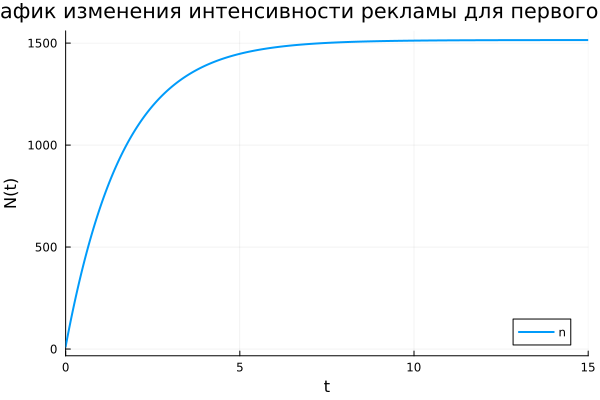
\includegraphics[width=0.7\textwidth,height=\textheight]{image/case1.png}

}

\caption{\label{fig-001}График первого случая}

\end{figure}%

Найдем решение для второго случая и построим его. Также найдем время,
когда производная принимает максимальное значение(рис.4)

\begin{figure}

\centering{


\includegraphics[width=0.7\textwidth,height=\textheight]{image/pic9.png}

}

\caption{\label{fig-001}Реализация в Julia}

\end{figure}%

В случае 2 мы видим, что кривая сначала движется так быстро, что
достигает максимума, отмеченного красной точкой, намного быстрее, чем в
случае 1(рис.5)

\begin{figure}

\centering{

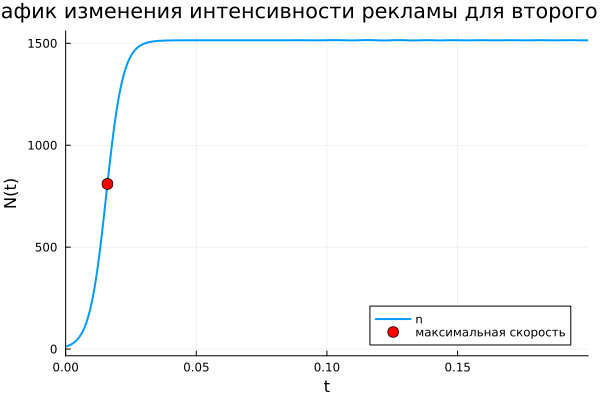
\includegraphics[width=0.7\textwidth,height=\textheight]{image/case2.png}

}

\caption{\label{fig-001}График второго случая}

\end{figure}%

Найдем решение для третьего случая и построим его. Также найдем время,
когда производная принимает максимальное значение(рис.6)

\begin{figure}

\centering{


\includegraphics[width=0.7\textwidth,height=\textheight]{image/pic11.png}

}

\caption{\label{fig-001}Реализация в Julia}

\end{figure}%

Из графика случая 3 видно, что максимальная скорость достигается уже при
t ≈ 0.02, что значительно быстрее, чем в случае 1 и 2, но медленнее, чем
в случае 2 (где t\_max ≈ 0.016).(рис 7 и 8)

\begin{figure}

\centering{


\includegraphics[width=0.7\textwidth,height=\textheight]{image/case3a.png}

}

\caption{\label{fig-001}График третьего случая}

\end{figure}%

\begin{figure}

\centering{

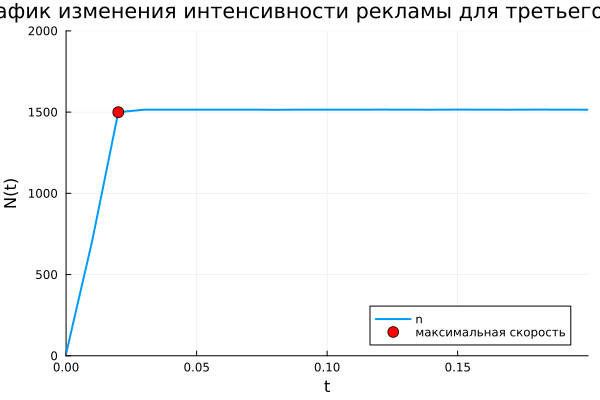
\includegraphics[width=0.7\textwidth,height=\textheight]{image/case3.png}

}

\caption{\label{fig-001}График третьего случая}

\end{figure}%

Мы сравним коэффициенты модели, используя график их изменения во
времени(рис.9)

\begin{figure}

\centering{


\includegraphics[width=0.7\textwidth,height=\textheight]{image/pic13.png}

}

\caption{\label{fig-001}Реализация в Julia}

\end{figure}%

Мы видим, что поначалу сарафанное радио более эффективно, чем платная
реклама, но со временем эффективность сарафанного радио снижается, и
платная реклама начинает доминировать(рис.10)

\begin{figure}

\centering{

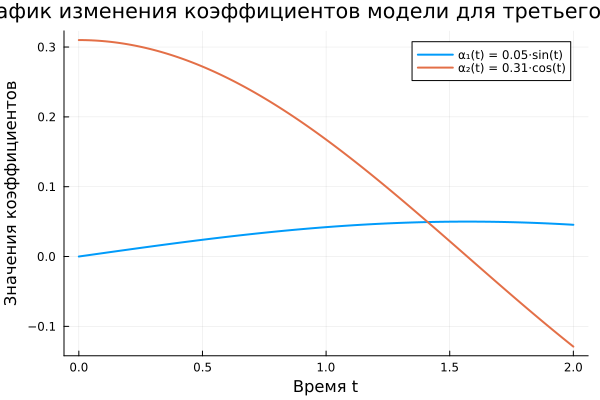
\includegraphics[width=0.7\textwidth,height=\textheight]{image/coefficients_case3.png}

}

\caption{\label{fig-001}График изменения коефициентов}

\end{figure}%

\section{Реализация в
Scilab}\label{ux440ux435ux430ux43bux438ux437ux430ux446ux438ux44f-ux432-scilab}

Я создала такую же модель с помощью scilab

'\,'\,'

// Случай 1 t1 = 0:0.1:15; x0 = 12; N = 1515;

function g = k1(t) g = 0.605; endfunction

function v = p1(t) v = 0.000015; endfunction

function xd = f1(t, x) xd = (k1(t) + p1(t)\emph{x)}(N - x); endfunction

x1 = ode(x0, 0, t1, f1);

scf(1); plot(t1, x1, \enquote*{b-}, \enquote*{LineWidth}, 2);
xlabel(\enquote{t}); ylabel(\enquote{N(t)}); title(\enquote{График
изменения интенсивности рекламы для первого случая});

// Случай 2 t2 = 0:0.0005:0.2;

function g = k2(t) g = 0.000025; endfunction

function v = p2(t) v = 0.205; endfunction

function xd = f2(t, x) xd = (k2(t) + p2(t)\emph{x)}(N - x); endfunction

x2 = ode(x0, 0, t2, f2);

// Нахождение максимальной скорости dev2 = {[}{]}; for i = 1:length(t2)
dev2(i) = (k2(t2(i)) + p2(t2(i))\emph{x2(i))}(N - x2(i)); end
{[}max\_dev2, idx\_max2{]} = max(dev2); t\_max2 = t2(idx\_max2);

scf(2); plot(t2, x2, \enquote*{r-}, \enquote*{LineWidth}, 2);
plot(t2(idx\_max2), x2(idx\_max2), \enquote*{ro}, \enquote*{MarkerSize},
8, \enquote*{MarkerFaceColor}, \enquote*{r}); xlabel(\enquote{t});
ylabel(\enquote{N(t)}); title(\enquote{График изменения интенсивности
рекламы для второго случая});

scf(3); plot(t2, dev2, \enquote*{g-}, \enquote*{LineWidth}, 2);
xlabel(\enquote{t}); ylabel(\enquote{dn/dt}); title(\enquote{График
изменения скорости рекламы для второго случая});

// Случай 3 t3 = 0:0.01:8;

function g = k3(t) g = 0.05*sin(t); endfunction

function v = p3(t) v = 0.31*cos(t); endfunction

function xd = f3(t, x) xd = (k3(t) + p3(t)\emph{x)}(N - x); endfunction

x3 = ode(x0, 0, t3, f3);

// Нахождение максимальной скорости dev3 = {[}{]}; for i = 1:length(t3)
dev3(i) = (k3(t3(i)) + p3(t3(i))\emph{x3(i))}(N - x3(i)); end
{[}max\_dev3, idx\_max3{]} = max(dev3); t\_max3 = t3(idx\_max3);

scf(4); plot(t3, x3, \enquote*{m-}, \enquote*{LineWidth}, 2);
plot(t3(idx\_max3), x3(idx\_max3), \enquote*{mo}, \enquote*{MarkerSize},
8, \enquote*{MarkerFaceColor}, \enquote*{m}); xlabel(\enquote{t});
ylabel(\enquote{N(t)}); title(\enquote{График изменения интенсивности
рекламы для третьего случая});

scf(5); plot(t3, dev3, \enquote*{c-}, \enquote*{LineWidth}, 2);
xlabel(\enquote{t}); ylabel(\enquote{dn/dt}); title(\enquote{График
изменения скорости рекламы для третьего случая});

// График коэффициентов (как в Julia рис. 4.4) t\_coeff = 0:0.001:2.0;
alpha1 = 0.05\emph{sin(t\_coeff); alpha2 = 0.31}cos(t\_coeff);

scf(6); plot(t\_coeff, alpha1, \enquote*{b-}, \enquote*{LineWidth}, 2);
plot(t\_coeff, alpha2, \enquote*{r-}, \enquote*{LineWidth}, 2);
xlabel(\enquote{Время t}); ylabel(\enquote{Значения коэффициентов});
title(\enquote{График изменения коэффициентов модели для третьего
случая}); legend(\enquote{α₁(t) = 0.05·sin(t)}, \enquote{α₂(t) =
0.31·cos(t)});

'\,'\,' Для первого случая(рис.11)

\begin{figure}

\centering{


\includegraphics[width=0.7\textwidth,height=\textheight]{image/pic1.png}

}

\caption{\label{fig-001}График первого случая}

\end{figure}%

Для второго случая получим график изменения интенсивности рекламы,
также, выбрав в качестве отображаемой функции производную, получим
график, на котором видна максимальная скорость изменения интенсивности
рекламы(рис 12 и 13)

\begin{figure}

\centering{


\includegraphics[width=0.7\textwidth,height=\textheight]{image/pic2.png}

}

\caption{\label{fig-001}График второго случая}

\end{figure}%

\begin{figure}

\centering{


\includegraphics[width=0.7\textwidth,height=\textheight]{image/pic3.png}

}

\caption{\label{fig-001}График изменения скорость}

\end{figure}%

Для третьего случая получим график изменения интенсивности рекламы,
также, выбрав в качестве отображаемой функции производную, получим
график, на котором видна максимальная скорость изменения интенсивности
рекламы(рис 14 и 15)

\begin{figure}

\centering{


\includegraphics[width=0.7\textwidth,height=\textheight]{image/pic4.png}

}

\caption{\label{fig-001}График второго случая}

\end{figure}%

\begin{figure}

\centering{


\includegraphics[width=0.7\textwidth,height=\textheight]{image/pic5.png}

}

\caption{\label{fig-001}График изменения скорость}

\end{figure}%

\chapter{Выводы}\label{ux432ux44bux432ux43eux434ux44b}

Выполнив эту лабораторную работу, построили математической модели
Эффективность рекламы.


\printbibliography


\end{document}
